\documentclass[../summary.tex]{subfiles}

\begin{document}
	
	\section{Wetenschapsfilosofie}
	
	\subsection{Rol van menselijke activiteit op klimaatverandering}
	
	We kunnen onszelf afvragen of en in welke mate de klimaatsverandering beïnvloed is door menselijke activiteit. Het antwoord op die vraag is door de jaren heen sterk veranderd door een betere kennis over het onderwerp als gevolg van wereldwijd klimaatonderzoek. Figuur \ref{fig:progressive-understanding-climate-change} toont de evolutie van deze kennis. Op dit moment is het zeker dat de atmosfeer, de oceaan en het land opgewarmd is door menselijke invloed, al was dit duidelijk niet altijd het geval.
	
	\begin{figure} [htbp]
		\centering
		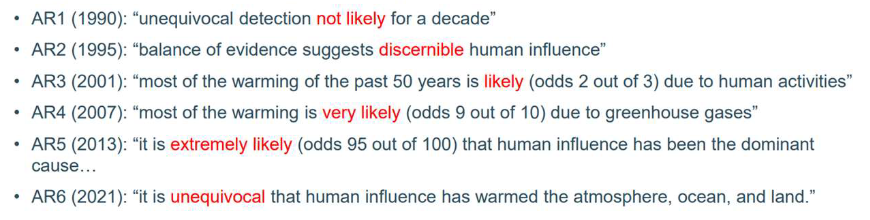
\includegraphics[width=1\linewidth]{images/progressive-understanding-climate-change.png}
		\caption{Evolutie van kennis over klimaatsverandering}
		\label{fig:progressive-understanding-climate-change}
	\end{figure}
	
	\subsection{Het Voorzorgsprincipe}
	
	De Verklaring van Rio uit 1992 stelt dat waar er een dreiging van ernstige of onomkeerbare schade is, het gebrek aan volledige wetenschappelijke zekerheid niet gebruikt mag worden als een reden om kostenefficiënte maatregelen om milieuschade tegen te gaan, uit te stellen.”. Dit is beter bekend als \textbf{het Voorzorgsprincipe}.
	\\\\
	We kunnen ons nu afvragen wat \textbf{volledige wetenschappelijke zekerheid} is. Het ideaaltype over wetenschap is gebaseerd op \textbf{rationele en betrouwbare kennis} en dus niet alleen maar intuïtief of emotioneel. Ten tweede kan wetenschap \textbf{veralgemeend} worden. Er kunnen geen uitzonderingen zijn en moet ook geldig zijn voor de toekomst. Het kan niet alleen anekdotisch of casuïstisch zijn en tijd en ruimte zijn uniform. Verder moet wetenschap \textbf{objectief} zijn en vrij zijn van waarden of belangen. Het ideaaltype van wetenschap is \textbf{coherent} opgebouwd en geen losse verzameling weetjes. Ten slotte moet er een \textbf{consensus in wetenschappelijke gemeenschap} zijn.
	
	\subsection{Demarcatiecriteria}
	
	\subsubsection{Demarcatiecriteria voor wetenschap}
	
	Vervolgens zullen we de criteria bespreken die wetenschap van niet-wetenschap kunnen onderscheiden. Dit zijn de zogenaamde \textbf{demarcatiecriteria} of afbakeningscriteria. Op het eerste zicht zou het gebruik van wiskunde en getallen een logisch criterium kunnen zijn. Er zijn echter ook een groot aantal niet-wetenschappelijke domeinen die getallen gebruiken (bv. puntentelling van een voetbalmatch). Aan de andere kant zijn er ook een aantal wetenschappelijke domeinen die geen getallen gebruiken (bv. psychologie). 
	\\\\
	Twee andere mogelijke criteria zijn de mogelijkheid om voorspellingen te maken en de mogelijkheid om met experimenten te werken. We kunnen ons dan wel afvragen hoe precies die experimenten moeten zijn. En wat doen we als er praktische of ethische bezwaren zijn tegen een bepaald experiment. We kunnen dus concluderen dat dit ook geen geschikte criteria zijn om wetenschap strikt te definiëren. 
	\\\\
	Een laatst mogelijke criterium is of het geverifieerd of gefalsifieerd kan worden. 
	
	\subsubsection{Verifieerbaarheid als demarcatiecriterium}
	
	De oorsprong van verifieerbaarheid als een afbakeningscriterium ligt in het "logisch empirisme". We kunnen naar wetenschap kijken als een verzameling ware zinnen. Dit kunnen empirische of logische waarheden zijn. We kunnen de zinnen ontleden in hun samenstellende delen en voor elk deel controleren of dat het verifieerbaar is of dat het een logische operator is.
	\\\\
	Een eerste manier om dit in de praktijk te doen, zou zijn om te controleren of het \textbf{actueel verifieerbaar} is. Dit kan in sommige gevallen praktische problemen veroorzaken (bv. als we de temperatuur van de zon zouden willen meten). Daarom kunnen we dit principe van verifieerbaarheid verzachten tot \textbf{principiële verifieerbaarheid}. Zelfs dit is in sommige gevallen nog te streng. Een andere manier om iets te verifiëren, zou kunnen zijn door te kijken naar de mogelijkheid om \textbf{principiële confirmeerbaarheid} te vinden. Dit is echter niet strikt genoeg. We zouden een middenweg moeten vinden tussen de twee. Bij het kijken naar de mogelijkheid om bevestiging te vinden, moeten we ook oppassen voor de \textbf{paradox van de confirmerende instantie}. Ik zal het volgende voorbeeld gebruiken om deze paradox te illustreren. Ik zou kunnen zeggen dat alle raven zwart zijn. In de vorm van een implicatie kan dit worden uitgedrukt als: Als iets een raaf is, dan is het zwart. Via contrapositie is deze verklaring equivalent aan: Als iets niet zwart is, dan is het geen raaf. In alle omstandigheden waarin de tweede verklaring waar is, is de eerste ook waar. Op dezelfde manier is in alle omstandigheden waarin de tweede verklaring onwaar is ook de eerste onwaar. Als ik nu bijvoorbeeld zeg dat mijn huisdier een zwarte raaf is, ondersteunt dit de hypothese dat alle raven zwart zijn. De paradox ontstaat wanneer dit proces wordt toegepast op de tweede verklaring. Bij het zien van een groene appel kan men waarnemen dat de groene appel niet zwart is en geen raaf is. Volgens dezelfde redenering is deze verklaring bewijs dat als iets niet zwart is, het geen raaf is. Maar aangezien (zoals hierboven) deze verklaring logisch equivalent is aan mijn verklaring dat alle raven zwart zijn, volgt daaruit dat het zien van een groene appel bewijs is dat de opvatting dat alle raven zwart zijn wordt ondersteund. Deze conclusie lijkt paradoxaal omdat het impliceert dat informatie over raven is verkregen door naar een appel te kijken. Een ander probleem van het gebruik van verifieerbaarheid als demarcatiecriterium is dat \textbf{empirische waarnemingen altijd selectief en constructief} zijn. Ten slotte zijn \textbf{samenzweringstheorieën} ook een probleem bij het proberen verifieerbaarheid als afbakeningscriterium te gebruiken.
	
	\subsubsection{Samenzweringstheorieën}
	
	Een samenzweringstheorie is een verklaring voor een gebeurtenis of situatie die beweert dat er sprake is van een samenzwering door machtige en sinistere groepen, vaak gemotiveerd door politieke redenen, wanneer andere verklaringen waarschijnlijker zijn. Typische argumenten voor deze theorieën zijn vervalste gegevens of corrupte peer review-processen. Samenzweringstheoretici geloven vaak dat 'niets zomaar gebeurt'. Het zijn vaak paniekzaaiers met een hyperkritische houding tegenover de mainstream media maar zijn zeer kritiekloos ten opzichte van hun eigen opvattingen. Hun theorieën worden ook vaak beïnvloed door politieke of commerciële belangen. De logica achter samenzweringstheorieën is dat als je iets vindt dat je samenzweringstheorie bevestigt, dan is je theorie bevestigd; maar aan de andere kant, als je niets vindt om je samenzweringstheorie te bevestigen, dan is er een samenzwering om het bewijs te verbergen, wat je samenzweringstheorie ook bevestigt. Dus, wat er ook gebeurt, je theorie is bevestigd.
	
	\subsubsection{Falsifieerbaarheid}
	
	We kunnen dus concluderen dat verifieerbaarheid en confirmeerbaarheid te laks zijn om als afbakeningscriterium te dienen. Een nieuw alternatief dat we zullen bestuderen, is falsifieerbaarheid. De belangrijkste promotor van deze alternatieve benadering is Karl Popper (1902 - 1994). Falsifieerbaarheid is gebaseerd op het feit dat je voor bijna alles bevestiging kunt vinden als je er in gelooft of er hard genoeg naar zoekt. Een wetenschappelijke theorie is sterker indien ze zodanig precies is dat de kans dat ze
	bevestigd wordt, zeer klein is. Wetenschappen moeten openstaan voor falsificatie. Ze moeten zelf aangeven welke gebeurtenissen (als ze ooit plaatsvinden) zouden aantonen dat je theorie onjuist is. Daarom zijn theorieën die niet openstaan voor falsificatie niet wetenschappelijk (de zogenaamde "pseudo-wetenschappen"). Door falsifieerbaarheid te gebruiken, gaat de wetenschap vooruit door middel van eliminatie, gissen en missen. 
	\\\\
	Er zijn enkele beperkingen gepaard met falsifieerbaarheid. Een theorie bestaat namelijk altijd uit een samenstelling van meerdere aannames. Hierdoor wordt het moeilijk om te weten welk deel van de theorie precies weerlegd wordt. Verder is falsificatie afhankelijk van een reeks veronderstellingen over de geldigheid van waarnemingen. Men gaat er vanuit dat de meetopstelling correct is de toestellen correct geijkt zijn. Men moet ook opletten voor "ad hoc hypothesen" die gebruikt kunnen worden om theorieën te beschermen tegen falsificatie. Er moet ook correct omgegaan worden met statistieken.
	\\\\
	Om Popper te citeren: "Wetenschap is een oneindige zoektocht. Er zijn geen definitieve
	theorieën. We hebben alleen hypothesen die nog niet weerlegd zijn." We zouden dus kunnen spreken van systematische twijfel als het om wetenschap gaat.
	
	\subsection{Kwaliteitsindicatoren voor wetenschappelijk werk}
	
	Er zijn een paar kenmerken die duiden op kwalitatief wetenschappelijk werk. De eerste is \textbf{openheid voor falsificatie}. Dit draagt bij aan je geloofwaardigheid en gaat tegen dogmatisme, fundamentalisme en samenzweringstheorieën in. Ten tweede moet wetenschappelijk werk een \textbf{verklarende kracht} hebben en de mogelijkheid om \textbf{voorspellingen} te maken. Een andere indicator van kwaliteit is \textbf{eenvoud}. Ten slotte moet wetenschappelijk werk ook \textbf{consistent} zijn met andere en aangrenzende vakgebieden.
	
	\subsection{Vooronderstellingen over wetenschap}
	
	We hebben de eigenschappen voor het ideaaltype over wetenschap al besproken. Hieruit volgen ook enkele vooronderstellingen over wetenschap. Zo verwachten we bijvoorbeeld dat wetenschap \textbf{louter beschrijvend} is. Het moet gaan over \textbf{feiten} en over \textbf{verbanden tussen feiten}. Verder zou wetenschap \textbf{voor iedereen hetzelfde en aanvaardbaar} moeten zijn. De wetenschapper moet ook handelen als een afstandelijke waarnemer. Dit houdt in dat er \textbf{scheiding van subject en object} is. Ten slotte moet wetenschap ook \textbf{waardevrij} zijn.
	\\\\
	We verwachten zekerheid en betrouwbaarheid van kennis en toch stellen we vast dat er toch nog veel onzekerheid is. Dit zou een aantal redenen kunnen hebben. De eerste reden zou \textbf{onwetendheid} kunnen zijn. Er zijn bepaalde zaken die we simpelweg (nog) niet weten. Als we naar het verleden kijken, zijn er ook zaken die we nu weten maar 10 of 20 jaar geleden nog niet. Dit zal naar de toekomst toe waarschijnlijk niet veranderen. Een tweede reden zou \textbf{onenigheid over data} kunnen zijn, al zal dit in de realiteit waarschijnlijk weinig voorvallen aangezien de data steeds is wat ze is. Er zou eerder sprake kunnen zijn van een \textbf{verschil in interpretaties}. Verder is \textbf{fraude} ook een mogelijke reden die tot onzekerheid in de wetenschap kan leiden. Bepaalde wetenschappers kunnen in het verleden hun meetresultaten aangepast hebben of enkel gunstige resultaten geselecteerd hebben om hun hypothese te bevestigen, al komt dit in de realiteit zeer zelden voor. Ten slotte zou er ook \textbf{inherente onzekerheid} aangegeven kunnen worden vanuit de wetenschap waarbij chaotische systemen zeer verschillende eindresultaten zullen teruggeven. We kunnen ons dus vragen beginnen stellen bij deze waardevrije wetenschap, al is dit iets waar we natuurlijk altijd naar kunnen blijven streven.
	
	\subsection{Waardevrije wetenschap}
	
	\subsubsection{Gustav Von Schmoller en Max Weber}
	
	Gustav Von Schmoller is een Duits economist en leider van een belangrijke economische strekking. Volgens Von Schmoller was de rol van economie als wetenschap om beleidsadviezen mee te geven. Volgens hem zijn diegene die de situatie het best kennen en begrijpen het meest geschikt om beleid te voeren. Dit is dus de taak van de wetenschappers. Max Weber is een intellectueel die zich onder ander bezig hield met filosofie, sociologie, theologie en economie. Hij ging sterk in tegen de visie van Von Schmoller. Volgens Weber was het niet de taak van de wetenschap om beleid te voeren maar om de wereld zo objectief mogelijk te beschrijven. Wetenschap moet waardevrij en zo neutraal en objectief mogelijk zijn. De theorie over waardevrije wetenschap die we zullen behandelen vertrekt grotendeels uit de theorie van Weber. 
	
	\begin{figure} [htbp]
		\centering
		\begin{subfigure}{0.3\linewidth}
			\centering
			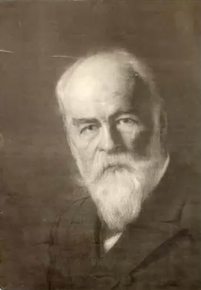
\includegraphics[width=\linewidth]{images/2-von-schmoller.png}
			\caption{Gustav Von Schmoller}
			\label{fig:von-schmoller}
		\end{subfigure}
		\begin{subfigure}{0.3\linewidth}
			\centering
			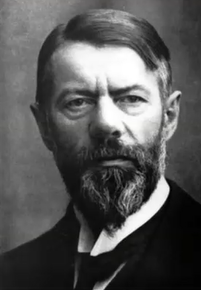
\includegraphics[width=\linewidth]{images/2-weber.png}
			\caption{Max Weber}
			\label{fig:weber}
		\end{subfigure}
			\caption{Gustav Von Schmoller (1838-1917) en Max Weber (1864-1920)}
		\label{fig:von-schmoller-weber}
	\end{figure}
	
	\subsubsection{Dualismen van Weber}
	
	Er zitten volgens Weber \textbf{3 dualismen} achter het idee van waardevrije wetenschap, namelijk het dualisme tussen \textbf{feiten en waarden}, het dualisme tussen \textbf{wetenschap en politiek} en het dualisme tussen \textbf{wetenschap en technologie}. We zullen vooral dit tweede dualisme bespreken aangezien dit nauw aansluit met de theorie van Weber.
	
	\subsubsection{Dualisme tussen wetenschap en politiek}
	
	Wetenschap en politiek zouden zich zo weinig mogelijk moeten inmengen. Zaken zijn waar of niet waar, onafhankelijk van het gegeven of ze in een politiek of religieus kraam passen of niet. In het verleden zijn er echter wel voorbeelden terug te vinden waarin er sprake is geweest van \textbf{politieke inmenging} in de wetenschap. 
	\\\\
	Zo geloofde Galileo Galilei na de uitvinding van de telescoop dat niet de aarde maar de zon in het centrum van het universum staat en dat de aarde rond de zon draait. Dit viel niet in goede aarde bij de machthebbers van toen. Indertijd geloofde men in een hiërarchisch kosmosbeeld met een duidelijk boven en beneden. Hierbij werd alles wat  op aarde gebeurde aangestuurd door de beweging van de sterren die in beweging werden gezet door een soort van godheid. Dit model kwam ook terug om de maatschappij te besturen met vanboven koningen en keizers en beneden de gewone mens, idem voor de Kerk met vanboven de paus en beneden de gewone gelovigen met de nodige tussenliggende structuren. Met kon deze maatschappijstructuur verantwoorden door te verwijzen naar de structuur die God in de kosmos gestoken had. Door dit in twijfel te trekken werd dit dus een bedreiging voor de machthebbers in de samenleving. 
	\\\\
	Een meer recent voorbeeld is dat van Trofim Lyssenko die zich bezig hield met erfelijkheid. Na de Russische revolutie hielden de aanhangers van het oude tsaristische regime vast aan het gegeven dat Adelheid erfelijk was, om zo hun oude status te behouden. Lyssenko kwam af met een andere interpretatie van erfelijkheid af die hier tegen in ging om zo dus ook zijn politieke tegenstanders ongelijk te geven. We kunnen dus stellen dat er voor een theorie gekozen is, niet omdat hij wetenschappelijk juist was (en dat bleek ze achteraf ook niet te zijn), maar omdat ze in een politiek kraam paste. 
	\\\\
	In onze huidige samenleving kunnen we ook \textbf{inmenging van bedrijven} zien. Zo zijn er voorbeelden van oliebedrijven die het onderzoek naar klimaatverandering proberen tegenhouden omdat dit een negatieve invloed op hun bedrijf zal hebben. 

	\begin{figure} [htbp]
		\centering
		\begin{subfigure}{0.3\linewidth}
			\centering
			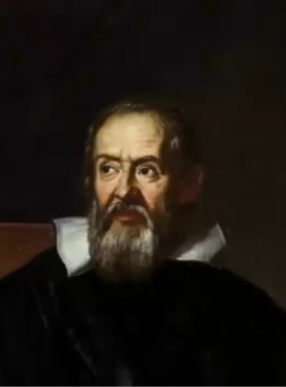
\includegraphics[width=\linewidth]{images/2-galilei.png}
			\caption{Galileo Galilei (1562-1642)}
			\label{fig:galilei}
		\end{subfigure}
		\begin{subfigure}{0.3\linewidth}
			\centering
			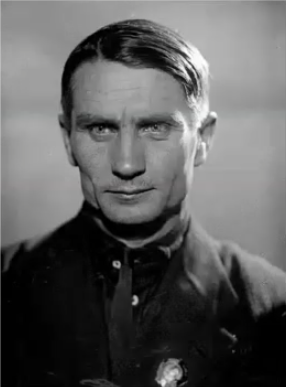
\includegraphics[width=\linewidth]{images/2-lyssenko.png}
			\caption{Trofim Lyssenko (1898-1976}
			\label{fig:lyssenko}
		\end{subfigure}
		\caption{Voorbeelden van politieke inmenging}
		\label{fig:politieke-inmenging}
	\end{figure}
	
	\subsubsection{Dualisme tussen feiten en waarden}
	
	Vervolgens kunnen we ook dieper ingaan op de dualiteit tussen feiten en waarden. \textbf{Feiten} zijn wat ze zijn. We kunnen ze beschouwen als een soort van onpartijdige scheidsrechter wanneer er discussie zou ontstaan. Men vertrekt vanuit de correspondentietheorie van waarheid. Dit houdt in dat waarheid afhangt van de overeenkomst tussen wat men kan waarnemen en wat wetenschappelijk beheerst wordt. De wetenschapper is een neutraal observator die de werkelijkheid enkel registreert met een objectivistische visie op de feiten.
	\\\\
	\textbf{Waarden} aan de andere kant kunnen wel partijdig en subjectief zijn. Er is in discussie dus geen externe, onpartijdige scheidsrechter mogelijk. Het is wel wenselijk dat er dialoog en verantwoording mogelijk is over de waarden. Wanneer er nu een beslissing gemaakt wordt, zal dit nooit enkel op basis van feiten gebeuren. In realiteit worden beslissingen altijd op basis van een combinatie van feiten en waarden gemaakt. 
	\\\\
	Het dualisme tussen feiten en waarden volgt ook duidelijk uit de taal die we voor beiden gebruiken. Voor feiten zal er een descriptieve of beschrijvende taal gebruikt worden, terwijl voor waarden met een prescriptieve of normatieve taal gebruikt wordt. In het Duits kunnen we het onderscheid maken tussen \textit{sein} en \textit{sollen}. Dit gebeurt in het Engels op dezelfde manier met \textit{is} en \textit{ought}. 
	\\\\
	In de praktijk is dit onderscheid tussen descriptieve en normatieve taal niet altijd duidelijk. Een goed voorbeeld hiervan is het gebruik van het woord \textit{normaal}. Dit is een woord dat meerdere betekenissen kan hebben. Een eerste betekenis is `wat kan uitgelegd worden op basis van kennis'. Verder kan het ook betekenen `wat statistisch veel voorkomt'. We kunnen ons dan wel de bedenking maken vanaf wanneer iets `abnormaal' is. Een derde betekenis van \textit{normaal} is `wat cultureel gebruikelijk is'. Dit kan echter wel diachroon (doorheen de tijd) en synchroon (op een bepaald moment) variëren. Deze mogelijke betekenissen zijn allemaal descriptief. We kunnen echter ook een vierde, normatieve betekenis vinden, namelijk `wat goedgekeurd wordt'.
	
	\subsection{Paradigma's en disciplinaire matrices}
	
	Een term die in de beschrijving van wetenschap vaak gebruikt wordt is die van zogenaamde \textbf{paradigma's}. Deze term kan verschillende betekenissen hebben. De eerste betekenis is die van paradigma's als leervoorbeelden, oftewel een soort van oefeningen die je moet doen als je een bepaalde discipline aan het aanleren bent. Een voorbeeld hiervan zijn vingeroefeningen in muziek - of typeles. In de wetenschap zal dit ook voorkomen, bijvoorbeeld als basisoefeningen in driehoeksmeting waarin je basisconcepten leert die je later in uitgebreidere oefeningen zult moeten toepassen en combineren. Later is dit concept uitgebreid tot een disciplinaire matrix.
	\\\\
	Een \textbf{disciplinaire matrix} bestaat uit de componenten die gebruikt worden wanneer je een bepaalde discipline gaat beoefenen. De eerste laag is die van de \textbf{metafysische componenten}. Die laag zal gaan over waar de wereld uit bestaat vanuit de discipline. In de chemie zullen dit atomen, moleculen en ionen zijn; in de elektriciteit zullen dit ladingen, weerstanden en spanningen zijn en in de economie uit huishouden, spaarders, producenten en investeerders. Aan deze laag hangt echter het risico van reductionisme vast. Dit risico houdt in dat je de wereld zult gaan herleiden tot wat je kent. De keerzijde hiervan is dat je zaken die niet bij je discipline horen zult gaan proberen forceren binnen je discipline of gewoon niet gaat erkennen. Een voorbeeld hiervan is wanneer men mensen vraagt om kaarten in te delen in een kaartspel, ze een zwarte harten zullen herleiden tot schoppen. 
	De volgende laag uit de disciplinaire matrix bestaat uit \textbf{definities, symbolen en wetten} en zal tussen gaan over namen, symbolen en voorstellingswijzen. We kunnen dit opnieuw toepassen op de voorbeelden uit de chemie, elektriciteit en economie. In de chemie houdt dit onder anderen het getal van Avogado, maar ook de termen pH, zuren en basen in; in de elektriciteit vallen zaken zoals de wet van Ohm en RC kringen hieronder en in de economie kunnen we de termen vraag/aanbod en het multiplicatoreffect aanhalen als voorbeelden voor deze laag. Deze laag is dus duidelijk afhankelijk van de vorige laag. We lopen hier ook opnieuw het risico dat we enkel die definities en symbolen (h)erkennen die bij ons systeem passen. 
	De derde laag binnen deze matrix is de laag van \textbf{gemeenschappelijke waarden en voorkeuren}. Dit kan dan gaan over hoe een bepaalde oplossing moet worden opgebouwd en opgesteld, over welke precisie we verwachten, over of we liever een grafische of een berekende oplossing willen of over wat we willen optimaliseren. 
	Een vierde laag bestaat uit \textbf{typische voorbeelden en oefeningen}. Opnieuw teruggrijpend naar het voorbeeld uit de chemie zou dit bijvoorbeeld titraties kunnen inhouden. In de thermodynamica zouden dit verschillende toepassingen van de Carnot -cyclus kunnen zijn. 
	\\\\
	Bij uitbreiding kunnen we ook denken aan bepaalde gewoontes die men binnen een bepaalde discipline heeft om bepaalde zaken aan te pakken zoals de keuze van instrumenten en metingen, maar ook eventuele politieke overtuigingen, titels en rituelen. Uit deze disciplinaire matrix volgt dus dat er ook aan wetenschappelijk werk een aantal keuzes, voorkeuren en waarden inherent zijn. Hieruit volgt dus ook opnieuw dat wetenschap misschien niet helemaal waardevrij zal zijn zoals Max Weber dat opperde. Er zullen altijd keuzes gemaakt moeten worden en aan deze keuzes zullen in de realiteit altijd bepaalde waarden verbonden zijn.
	\\\\
	We kunnen dus concluderen dat paradigma's en disciplinaire matrices instrumenten aanreiken om toestanden te herkennen en benoemen en geldige oplossingen uit te werken. Ze maken communicatie mogelijk in de wetenschappelijke gemeenschap aangezien je pas kan communiceren als je voldoende vertrouwd bent met de begrippen uit een bepaalde discipline. Verder houdt een paradigma ook een belofte van succes in omdat een paradigma toe zou moeten laten om een bepaald probleem op te lossen. De keerzijde hieraan is dat wanneer dit niet het geval is dit direct in de schoenen van de onderzoeker geschoven zal worden. Als men op een bepaald moment op een probleem botst waarvoor men geen oplossing vindt, kan dit eventueel ook tot een paradigmawissel leiden waarbij men tot een andere manier van werken moet komen waarbij men plots andere dingen moet geloven. Voorbeelden hiervan zijn Copernicus met zijn manier van denken over de opbouw van het heelal, Darwin met zijn evolutietheorie en Einstein met zijn relativiteitstheorie en kwantumfysica. Een paradigmawissel verandert de manier waarop je de wereld begrijpt.
	\\\\
	Een ander voorbeeld van zo een paradigmawissel is de klimaatsverandering. Er is een soort van bewustwording ontstaan waarbij men rekening houdt met andere relevante parameters en meer onderlinge afhankelijkheden.
	
	
	
\end{document}